\cotefile{136}
\scanpage{220}
% slanted
\margin{De Rham P.D.}

\textcircled{3} Sur $\Gamma^*M\otimes\Lambda^*M$ \deleted{(algèbre bigraduée)} il y a un seul op. $d$ qui soit
\deleted{a) $A$ linéaire} a) une \inserted{anti}dérivation si \deleted{$\Gamma^*(M)$ de degrés pairs et $\Lambda^1M$ de degré impair}
\inserted{$A$-algèbre graduée,} b) \inserted{antidérivation de degré 1} compatible avec les puiss. divisées sur $(\Gamma^*M)^+$ i.e. $d(x^{(i)})=x^{(i-1)}\,dx$, et
\unsure{c)} $d$ est nulle sur $\Lambda^1M$, et sur $\Gamma^1 M$ c'est l'isom can $\Gamma^1 M\longrightarrow\Lambda^1 M$.
Alors $d$ satisfait $d^2=0$, et applique $\Gamma^p\otimes\Lambda^q$ dans $\Gamma^{p\unsure{-|+}1}\otimes\Lambda^{q+1}$. Il est $\Lambda^*M$-linéaire.
C'est aussi \unsure{du|dit|le} ``complexe de De Rham à puissances divisées'' de la $A$-algèbre à p.d. $\Gamma^*M$ (avec son idéal $\Gamma^+M$).
\margin{? $\big\{$}
Si $M$ est plat sur $A$, alors on a (\unsure{graduant|gradué} par le degré de $\Lambda^*$)
\[
 H^{\unsure{*|i}}_{\mathrm{DR\,p.d.}}(\Gamma^*(M)\otimes\Lambda^* M)
 \simeq\begin{cases}0&\text{si }i\ne0\\
 \underset{\substack{\rotatebox{90}{$\simeq$}\\\Gamma^0\otimes\Lambda^0}}{A}&\text{si }i=0\end{cases}
\]

% slanted
\margin{Koszul P.D.}

\textcircled{4} Sur $\Gamma^*M\otimes\Lambda^*M$, il y a un seul op. $\delta$ qui soit
a) dérivation de \inserted{$A$-}algèbre graduée b) compatible avec p.d. sur $\Gamma^+(M)$ ($d(x^{(i)})=x^{(i-1)}dx$ si $x\in\Gamma^+$).
c) nulle sur $\Gamma^1 M$ \deleted{(donc sur $\Gamma^*M$ \unsure{entier})} et induisant sur $\Lambda^1M$ l'isom $\Lambda^1M\longrightarrow\Gamma^1M$.
\deleted{Si $M$ \unsure{libre} \inserted{plat} sur $A$, et si $A$ de \unsure{caractéristique}} \inserted{Alors $\delta^2=0$, il applique $\Gamma^p\otimes\Lambda^q$ dans $\Gamma^{p+1}\otimes\Lambda^{q-1}$,} \inserted{est $\Gamma^*M$-linéaire.}
Ecrivant les degrés en bas, si $M$ est plat \inserted{(inutile)} sur $A$ \deleted{\unsure{$M$}} de car. $0$, on a
\[
 H_i^{\mathrm{Kos\,p.d.}}(\Gamma^*M\otimes\Lambda^*M)\simeq
 \begin{cases}0&\text{si }i\ne0\\
 \underset{\substack{\rotatebox{90}{$\simeq$}\\\Gamma^0\otimes\Lambda^0}}{A}&\text{si }i=0\end{cases}
\]

Si $A$ de car $p>0$, $M$ plat, on doit avoir une histoire d'\unsure{opérations|opération} de Cartier\unsure{...}.

% archive sheet number: 219

\scanpage{221}
Relations entre les 4 complexes, et fonctorialités.

Les \deleted{complexes} algèbres différentielles sont \unsure{fonctorielles|fonctoriels} en $(A,M)$. Pour $A$ fixé, $M$ variable, elles transforment sommes en produit tensoriel (d'où, pour chacune, application diagonale compatible avec \deleted{$d$ ou $\delta$} la différentielle), et commutent aux \uline{$\lim$} filtrantes.

L'hom can. d'algèbres (fonctoriel en $A,M$)
\diagram{\begin{tikzcd}[ampersand replacement=\&,column sep=large]
 \operatorname{Sym}^*M\otimes\Lambda^*M \arrow[r]\arrow[d,equal] \& \Gamma^*M\otimes\Lambda^*M \arrow[d,equal]\\
 C^*_{\mathrm{DR}}\operatorname{Sym}^*M \arrow[r] \& C^*_{\mathrm{DR\,p.d.}}(\Gamma^*M)
\end{tikzcd}}
est compatible avec les différentielles $d$. (C'est un isom \deleted{pour} si $A$ de car $0$ (réciproque vraie si \deleted{$A$} $M$ libre de rang $>0$), donc le calcul de coh. dans 1 est contenu dans celui de 3. [ce dernier se fait en réduisant au cas où \deleted{$A$}$M$ est libre de t.f. par Lazard, puis par Künneth au cas $M$ libre de rang $1$, auquel cas c'est trivial].

L'hom can. d'algèbres
\[
 \operatorname{Sym}^*M\otimes\Lambda^*M\unsure{\relbar|\longrightarrow}\Gamma^*M\otimes\Lambda^*M
\]
est aussi compatible avec les opérateurs diff. $\delta$. \deleted{\unsure{Comme} \unsure{lemme}} \deleted{\unsure{C'est}} Procédant comme dessus, le calcul d'homologie de (4) est ramené à celui de (2), qui peut se traiter par la $=$ méthode que pour (1).

La \uline{définition} de \unsure{l'op.|opér.} $\delta$ dans (2) et (4) peut d'ailleurs se ramener à un cas plus général de Koszul: si $S$ est un anneau comm, $M$ un $S$-module, \deleted{\unsure{libre}} et $\varphi\colon M\to S$ une forme

% archive sheet number: 220

\scanpage{222}
linéaire sur $\mathcal M$, on trouve une unique antidérivation $\delta$ de $\Lambda^*\mathcal M$ qui sur $\Lambda^1\mathcal M$ se réduise à $\varphi$, et on a $\delta^2=0$. (N.B. On a $H_0(\Lambda^*\mathcal M,\delta)=S/\varphi(\mathcal M)$, et si $\mathcal M$ est libre de t.f., alors $H_i(\Lambda^*\mathcal M,\delta)=0$ pour $i\ne0$ sss $\mathcal M\longrightarrow S$ est ``transversal'' -- il suffit p.ce. qu'une base \unsure{au moins|donnée} de $\mathcal M$ définisse une suite \uline{$S$-régulière}, et c'est aussi néc. si $S$ noeth et \deleted{\unsure{le}} $\varphi(\mathcal M)\subset\operatorname{rad} S$)
Ceci dit, on obtient les complexes (2) et (4) en prenant respectivement $S=\operatorname{Sym}^* M$ ou $S=\Gamma^*M$, $\mathcal M=M\otimes_A S$, et en prenant l'hom $\mathcal M\to S$ \deleted{\unsure{la}} dont la restriction à $M$ est l'hom can $M\xrightarrow{\sim}\deleted{\operatorname{Sym}^1M\subset S}\inserted{S^1\subset S}$ \deleted{\unsure{resp. $\Gamma^1M$}} ($S^1=\operatorname{Sym}^1 M$ resp $\Gamma^1 M$).

Les opérateurs $d\delta,\delta d$ dans $\operatorname{Sym}^*\otimes\Lambda^*$ resp $\Gamma^*\otimes\Lambda^*$ ne sont pas bien jolis, mais on voit de suite (tout \unsure{anticrochet|anticommutateur} des antidérivations étant une dérivation) que
\[
 \theta=d\delta+\delta d
\]
est une dérivation, \deleted{et} \deleted{qui dans le cas $S^{\unsure{1|*}}=\Gamma^*$ est compatible aux p.d.} ne changeant \deleted{\unsure{par} le} le bidegré, et qui sur \deleted{\unsure{$S^1$}} $S^1=\operatorname{Sym}^1$ ou $\Gamma^1$ et sur $\Lambda^1$ est l'identité; \inserted{de plus si $S^*=\Gamma^*$, il est compatible aux puiss. div. sur $\Gamma^*$.} Donc on en conclut facilement que a lieu
\[
 \boxed{(d\delta+\delta d)x=\theta x=nx}\qquad
 \substack{x\text{ de degré }\underline{\text{total}}\text{ }n\\ \text{i.e. }x\in\displaystyle\sum_{\substack{p+q=n\\\unsure{p,q\geq0}}}S^p\otimes\Lambda^q}
\]
Cela montre donc que si $A$ est de car. zéro (donc $n$ inversible $\forall\,n>0$) alors $H^{n}_{\mathrm{DR}}(S^*\otimes\Lambda^*)$ et $H^{\mathrm{Kosz}}_{n}(S^*\otimes\Lambda^*)$ ($S^*$ étant $\operatorname{Sym}^*\simeq\Gamma^*$) est nul si \deleted{\unsure{$d$}} $n>0$ (sans hyp. de platitude!). Plus gén., $H^n_{\mathrm{DR}}$ et $H_n^{\mathrm{Kosz}}$ sont nuls pour tout $n$ tel que $n.1_A$ inv. dans $A$.
\margin{$\Vert$}

% archive sheet number: 221

\scanpage{223}
Revenant au cas $A$ de car. 0, que peut on dire de $H^0_{\mathrm{DR}}$ et $H^{\mathrm{Kosz}}_0$ ? Pour $H_0$, on sait déjà que c'est $\simeq A$, est-il vrai que l'hom évident $A\longrightarrow H^0_{\mathrm{DR}}$ est aussi un isom ?\,\deleted{\unsure{tel}} i.e. que $\unsure{\forall|H}\ f\in\operatorname{Sym}^*(M)$ tel que $df=0$ soit \deleted{nulle} une constante, ? i.e. \inserted{si $h>0$,} $f\in\operatorname{Sym}^{\unsure{h|k}}(M)$, $n>0$ et $\underset{\substack{\rotatebox{90}{$\in$}\\(\operatorname{Sym}^{h-1}M)\otimes M}}{df}=0\implies f=0$, i.e. $\operatorname{Sym}^hM\xrightarrow{d}(\operatorname{Sym}^{h-1}M)\otimes\underset{\substack{\rotatebox{90}{$\simeq$}\\\Lambda^1M}}{M}$ est injectif?
\margin{\unsure{?}}
Or composant avec $\operatorname{Sym}^{h-1}(M)\,\underset{\substack{\rotatebox{90}{$\simeq$}\\\operatorname{Sym}^1M}}{\deleted{\otimes M}}\xrightarrow{\delta}\operatorname{Sym}^hM$ on trouve la multiplication par $k$ (car $\theta=d\delta+\delta d$ est égal à $\delta d$ sur $\operatorname{Sym}^k M$ puisque $\delta$ y est nul), donc inj, ok (Plus gén, ceci marche si $k$ inv. dans $A$.)

\uline{Dualité} Supposons $M$ et $M'$ deux $A$-modules accouplés vers $A$,
\[
 M\otimes M'\unsure{\relbar|\longrightarrow} A
\]
alors on en conclut des accouplements (\unsure{degré|degrés} par degré)
\[
 \begin{aligned}
 \operatorname{Sym}^* M\times\Gamma^*M'&\relbar A\\
 \Lambda^*M\times\Lambda^*M'&\relbar A
 \end{aligned}
\]
qui est une dualité parfaite si $M$ est proj de t.f. et $M'$ s'identifie à son dual. On en conclut des accouplements.
\[
 \deleted{\operatorname{Sym}}\ S^{\unsure{+|*}}\Lambda^*(M)\times\Gamma^*\Lambda^*(M')\longrightarrow A
\]
Ceci posé, on vérifie que les op. $d_M$ et $\delta_{M'}$, $\delta_M$ et $d_{M'}$ sont \deleted{\unsure{duaux}} en transposition pour cet accouplement.
D'ailleurs, on vérifie aussi que l'op. de multiplication d'un côté est en dualité avec l'op. de comultiplication de l'autre. Donc dans le cas de la dualité parfaite, les opérations $d_M$ et $\delta_{M'}$, $\delta_M$ et $d_{M'}$, multiplication et comultiplication, se déterminent mutuellement.

% archive sheet number: 222

\scanpage{224}
% printed form
% Reverse-side computer print visible through the paper; read in reflected order.
\texttt{\unsure{//***} CRAY2 \unsure{1324} \illegible{2}}
\figure{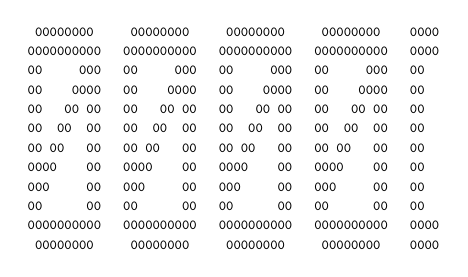
\begin{tikzpicture}[x=1pt,y=1pt,every node/.style={anchor=west,inner sep=0pt,font=\tiny\ttfamily}]
\node at (0,0) {~00000000~~~~~00000000~~~~~00000000~~~~~00000000~~~~\unsure{0000}};
\node at (0,-7) {0000000000~~~0000000000~~~0000000000~~~0000000000~~~\unsure{0000}};
\node at (0,-14) {00~~~~~000~~~00~~~~~000~~~00~~~~~000~~~00~~~~~000~~~\unsure{00}};
\node at (0,-21) {00~~~~0000~~~00~~~~0000~~~00~~~~0000~~~00~~~~0000~~~\unsure{00}};
\node at (0,-28) {00~~~00~00~~~00~~~00~00~~~00~~~00~00~~~00~~~00~00~~~\unsure{00}};
\node at (0,-35) {00~~00~~00~~~00~~00~~00~~~00~~00~~00~~~00~~00~~00~~~\unsure{00}};
\node at (0,-42) {00~00~~~00~~~00~00~~~00~~~00~00~~~00~~~00~00~~~00~~~\unsure{00}};
\node at (0,-49) {0000~~~~00~~~0000~~~~00~~~0000~~~~00~~~0000~~~~00~~~\unsure{00}};
\node at (0,-56) {000~~~~~00~~~000~~~~~00~~~000~~~~~00~~~000~~~~~00~~~\unsure{00}};
\node at (0,-63) {00~~~~~~00~~~00~~~~~~00~~~00~~~~~~00~~~00~~~~~~00~~~\unsure{00}};
\node at (0,-70) {0000000000~~~0000000000~~~0000000000~~~0000000000~~~\unsure{0000}};
\node at (0,-77) {~00000000~~~~~00000000~~~~~00000000~~~~~00000000~~~~\unsure{0000}};
\end{tikzpicture}}

\figure{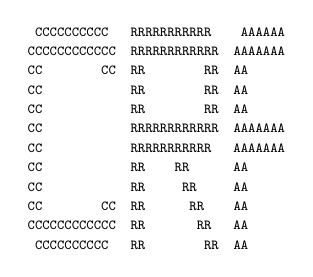
\begin{tikzpicture}[x=1pt,y=1pt,every node/.style={anchor=west,inner sep=0pt,font=\tiny\ttfamily}]
\node at (0,0) {~CCCCCCCCCC~~~RRRRRRRRRRR~~~~AAAAAA};
\node at (0,-7) {CCCCCCCCCCCC~~RRRRRRRRRRRR~~AAAAAAA};
\node at (0,-14) {CC~~~~~~~~CC~~RR~~~~~~~~RR~~AA};
\node at (0,-21) {CC~~~~~~~~~~~~RR~~~~~~~~RR~~AA};
\node at (0,-28) {CC~~~~~~~~~~~~RR~~~~~~~~RR~~AA};
\node at (0,-35) {CC~~~~~~~~~~~~RRRRRRRRRRRR~~AAAAAAA};
\node at (0,-42) {CC~~~~~~~~~~~~RRRRRRRRRRR~~~AAAAAAA};
\node at (0,-49) {CC~~~~~~~~~~~~RR~~~~RR~~~~~~AA};
\node at (0,-56) {CC~~~~~~~~~~~~RR~~~~~RR~~~~~AA};
\node at (0,-63) {CC~~~~~~~~CC~~RR~~~~~~RR~~~~AA};
\node at (0,-70) {CCCCCCCCCCCC~~RR~~~~~~~RR~~~AA};
\node at (0,-77) {~CCCCCCCCCC~~~RR~~~~~~~~RR~~AA};
\end{tikzpicture}}

\diagram{\(\begin{array}{llllll}
\texttt{****A}&\texttt{START}&\texttt{JOB}&\texttt{\unsure{1324|324}}&\texttt{CRAY2}&\texttt{ROOM}\ \unsure{1}\\
\texttt{****A}&\texttt{START}&\texttt{JOB}&\texttt{1324}&\texttt{CRAY2}&\texttt{ROOM}\ 1\\
\texttt{****A}&\texttt{START}&\texttt{JOB}&\texttt{1324}&\texttt{CRAY2}&\texttt{ROOM}\ 1\\
\texttt{****A}&\texttt{START}&\texttt{JOB}&\texttt{1324}&\texttt{CRAY2}&\texttt{ROOM}\ 1\\
\texttt{****A}&\texttt{START}&\texttt{JOB}&\texttt{1324}&\texttt{CRAY2}&\texttt{ROOM}\ 1\\
\texttt{****A}&\texttt{START}&\texttt{JOB}&\texttt{1324}&\texttt{CRAY2}&\texttt{ROOM}\ 1
\end{array}\)}

\texttt{DERNIERE MISE A JOUR \unsure{DE|DU} JOURNAL : \unsure{11-08-82}}\\
\texttt{ATTENTION \unsure{.............}}

\texttt{\unsure{J|1}\hspace{1em}1. UNE MODIFICATION SYSTEME NOUS CONTRAINDRA A DETRUIRE}\\
\texttt{J\hspace{2em}LE CONTENU DU DISQUE SPOOL LE MARDI 17 AOUT A \unsure{8|4} HEURES}\\
\texttt{J\hspace{2em}VEUILLEZ RECUPERER VOS SORTIES EN ATTENTE AVANT CETTE}\\
\texttt{J\hspace{2em}DATE. MERCI DE VOTRE COMPREHENSION.}\\
\texttt{J\hspace{1em}2. UN ARRET EXCEPTIONNEL POUR PREPARER L'ARRIVEE DE NOUVE\unsure{L}}\\
\texttt{J\hspace{2em}UNITES AURA LIEU DU VENDREDI 20 AOUT A 17H 30 AU LUNDI}\\
\texttt{J\hspace{2em}23 AOUT A 8H.}

% archive sheet number: 223

\scanpage{225}
% slanted
\margin{Feuille volante paumée ...}

\uline{Prop 6} Soit $\unsure{\mathcal B|B|\mathfrak B}$ une catégorie $k$-lin karoubienne. Alors le foncteur
\[
 ND_\bullet\colon\mathcal B_*^{\deleted{\unsure{*|\widehat{\ }}}}\longrightarrow\mathcal B_\bullet
\]
est donné (à isom can. près) par
\[
 ND_i(L_*)\simeq\operatorname{Hom}_{k,*}(\underbrace{\Lambda^i\unsure{\Phi|\mathscr L|\mathfrak L}_*}_{\Phi^i_\bullet},L_*)
\]
(pour la définition du $\operatorname{Hom}_{k,*}$, cf pag. 3, 5), \deleted{l'opérateur différentiel étant \unsure{les|la}} 
\[
 ND_\bullet(L_*)\simeq\operatorname{Hom}_{k,*}(\underbrace{\Lambda^\bullet\Phi_*}_{\Phi^\bullet_*},L_*)
\]
l'opérateur diff. sur $ND_\bullet(L_*)$ provient de l'op. différentiel sur \unsure{$T_*1$|Tout|$T_*$ et} sur $\Lambda^\bullet\Phi_*$.

En effet, \deleted{\unsure{comme}} \deleted{\unsure{on a pour}} soit $L_\bullet=ND_\bullet(L_*)$, et \deleted{\unsure{soit}} $\Phi(i)_\bullet=ND_\bullet(\deleted{\Phi}\Lambda^i\Phi_*)$, alors on a par \inserted{\unsure{la corresp.|l'équiv.|la symétrie} de \unsure{Dold, Puppe|Dold-Puppe}}
\[
 \operatorname{Hom}_{k,*}(\Lambda^i\Phi_*,L_*)\simeq\operatorname{Hom}_{k,\bullet}(\Phi(i)_\bullet,L_\bullet)
\]
Or $\Phi(i)_\bullet=C_\bullet^{i-1}$ pour $i\geq1$ (prop 4), et on \inserted{$\Phi(0)_\bullet=k$ placé en degré 0} a bien
\[
 \left\{\begin{aligned}
 \operatorname{Hom}_{k,\bullet}(C_\bullet^{i-1},L_\bullet)&\simeq L_i\quad(i\geq1)\\
 \operatorname{Hom}_{k,\bullet}(\unsure{(}k[0]_\bullet,L_\bullet)&\simeq L_0
 \end{aligned}\right.
\]
et il reste à faire de petites vérifications de compatibilité \unsure{...}.

\uline{Cor} Le foncteur $ND^\bullet\colon\mathcal B^*\to\mathcal B^\bullet$ s'explicite comme
\[
 ND^\bullet(L^*)\simeq\Lambda^\bullet\Phi_*\otimes_{k,*}L^*.
\]
[où pour un $M_*\in\mathrm{Ab}_{k*}$ et $L^*\in\mathcal B^*$,
$M_*\otimes_{k*}L^*$ désigne l'objet de $\uline{\operatorname{Hom}}(\mathcal B,(\unsure{Abgr|\mathrm{Ab}}))$
\[
 b\longmapsto\operatorname{Hom}_{\mathrm{Ab}_{k*}}(M_*,\operatorname{Hom}_{\mathcal B}(L^*,b))]
\]
\margin{$\big|$}

Il suffit d'appliquer la prop. 6 à $\mathcal B^\circ$.

% archive sheet number: 224

\scanpage{226}
% slanted
\margin{cette formule a un sens et est \unsure{vraie|vrai} sans supposer $\mathcal B$ karoubienne}

\[
 F(x)\simeq\operatorname{Hom}_k^*(\alpha^*(x),\underset{\substack{\rotatebox{90}{$=$}\,\mathrm{déf}\\ F(\mathbb C^*)}}{C_F^*})\quad\deleted{\unsure{*k}}
\]
où la définition du $\operatorname{Hom}^*$ se fait comme dans la prop. 3.

\deleted{\diagram{\begin{tikzcd}[ampersand replacement=\&,column sep=small]
 F(x)\otimes\alpha^{[n]}(x)\arrow[r]\& C_F^{[n]}\arrow[d,equal]\\
 \operatorname{Hom}(x,C^{[n]})\arrow[u,equal]\& F(\mathbb C^{[n]})
\end{tikzcd}}
% slanted
\margin{\unsure{par définition|par définitions} de $\alpha^*$ \deleted{et $DP$} $\alpha^*$ est \deleted{\unsure{de $DP$}} la commutation de $DP$ aux foncteurs \unsure{add.|std.|etc.}}
On procède comme pour la prop. 3 pour définir la flèche dans $\widehat{\mathcal B}$, et pour montrer que c'est un iso, on se ramène au cas $x$ de la forme $\mathbb C^{i}_{\unsure{*|\bullet|\xi}}$, il faut prouver qu'alors
\[
 F(\mathbb C^i)=C^i\longrightarrow\operatorname{Hom}_k^*(\unsure{\alpha^*},\mathbb C^\bullet)
\]}

En effet, on trouve \deleted{\unsure{tout}} de suite que si $K^\bullet\in\mathrm{Ab}_k^\bullet$, $C^\bullet\in\mathcal B^\bullet$, $K^*=DP(K^\bullet)$ et $C^*=DP(K^\bullet)$, alors on a un iso. can. bifonctoriel dans $\widehat{\mathcal B}$
\[
 DP\colon\operatorname{Hom}_k^\bullet(K^\bullet,C^\bullet)\simeq\operatorname{Hom}_k^*(K^*,C^*),
\]
et on conclut par prop 3.

\deleted{\uline{Prop 6} \textcircled{*} Le foncteur
\[
 ND\colon\mathrm{Ab}_{k*}\longrightarrow\mathrm{Ab}_{k\bullet}
\]
est donné par
\[
 (ND)(L_*)\simeq\operatorname{Hom}_{k,*}(\unsure{\mathbb C|C}_*^\bullet,L_*)
\]
i.e.
\[
 ND(L_*)_i\simeq\operatorname{Hom}_{k,*}(\underset{\substack{\rotatebox{90}{$=$}\\\Lambda^{i\unsure{+1}}\Phi_*}}{C_*^i},L_*)\quad\text{pour }i\geq0
\]
l'hom \inserted{bord} $ND(L_*)_i\to ND(L_*)_{i-1}$ $(i\geq1)$ étant le transposé de $C_*^{i-1}\longrightarrow C_*^i$.}

% archive sheet number: 225

\scanpage{227}
Quelques calculs d'homotopie

Soit $k$ un anneau de base (comm). $\Phi_*=\Phi_*^k$ \deleted{\unsure{$k$}} le $k$-module $\tfrac12$ simplicial $I\longmapsto k^I$ $k_*$ le $k$-module $\tfrac12$ \unsure{simpl|simpl.} const défini par $k$, $I\longmapsto k$. On a une application diagonale
\[
 k_*\longrightarrow\Phi_*
\]
d'où un quotient
\[
 \Psi_*=\Phi_*/k_*\colon I\longmapsto k^I/k
\]

\uline{Proposition} 1 \quad $\Phi_*$ est homotope à 0 \deleted{\unsure{$0_k$}} (\inserted{i.e. au $k$-}\deleted{module} $\tfrac12$ simplicial 0)

Par le \unsure{topos|topo|yoga} de Puppe-Dold, il suffit de voir que le complexe de chaînes $\Phi_*^!$ associé \deleted{$\Phi$} à $\Phi$ est homo à 0. Pour ceci, on se rappelle que a
\[
 \Phi_n^{\unsure{!|\bullet}}=\{x\in\Phi_n\mid\partial_1^*(x)=\cdots=\partial_n^*(x)=0\}
\]
\deleted{d'où} aussitôt
\[
 \Phi_n^!=\begin{cases}0&\text{si }n\geq2\\ k&\text{si }n=0,1\end{cases}
\]
l'op. \deleted{\unsure{cob|co}} bord
\[
 \partial=\partial_0\colon\underset{\substack{\rotatebox{90}{$\simeq$}\\k}}{\Phi_1^!}\longrightarrow
 \underset{\substack{\rotatebox{90}{$\simeq$}\\k}}{\Phi_0^!}
\]
étant l'identité, d'où la conclusion

\uline{Corollaire 1.1} Pour tt foncteur $F\colon\operatorname{Mod}(k)\longrightarrow C$ ($C$ une catégorie) $F(\Phi_*)$ est homotope à $F(0)$. En particulier
\[
 \left\{\begin{aligned}
 \Lambda_k^{\unsure{*|i}}\Phi_*\,\inserted{(\Gamma_k^i\Phi_*,\operatorname{Sym}_k^i\Phi_*)}
 &\text{ est homotope à }\Lambda_k^i(0)\,\inserted{(\Gamma_k^i(0),\operatorname{Sym}_k^i(0))}
 =\begin{cases}0&\text{si }i\ne0\\(k)_*&\text{si }i=0\end{cases}\\
 \deleted{\Gamma_k^i\Phi_*}&\deleted{\longrightarrow\Gamma_k^i(0)=
 \left\{\substack{0\ \text{si }i\ne0\\k_*\ \text{si }i=0}\right.}
 \end{aligned}\right.
\]

\uline{Corollaire} 1.2. Les groupes d'homotopie de $\Psi_*=\Phi_*/k_*$ sont
\[
 \pi_i(\Psi_*\,\deleted{/k_*})\simeq\pi_{i-1}(k_*)\simeq
 \begin{cases}0&\text{si }i\ne1\\ k&\text{si }i=1\end{cases}
\]
En d'autres termes, $\Psi_*\deleted{/k_*}$ est un $K_*(k,1)$
\margin{$\big[$}
[En fait, on a $(\Psi_*^!\deleted{/k_*^!})^!=$ complexe réduit à $k$ placé en degré 1.

On conclut de ceci:\deleted{\unsure{et du topos de décalage que|et du yoga de Dold-Puppe}}

\uline{Corollaire} 1.\unsure{3|2}. \quad $\pi_j(\Lambda^i(\Phi_*/k_*))\simeq\begin{cases}0&\text{si }j\ne i\\k&\text{si }j=i\end{cases}$

(i.e. $\Lambda^i\Phi_*/k_*$ est un $K_*(k,i)$).

% archive sheet number: 226

\scanpage{228}
\mspage{- 192 -}\hfill IX

14.2. \uline{Relations de l'homomorphisme} $i\colon\underline M_K\longrightarrow\mathbb G_K$ \uline{avec la monodromie}. Soit $n$ un entier $>0$. On déduit alors de la suite exacte (14.1.7), via la suite exacte des $\underline{\operatorname{Ext}}^i(\mathbb Z/n\mathbb Z,-)$ sur le site des espaces rigide-analytiques au-dessus de $K$, une suite exacte canonique (compte tenu du fait que $\underline M_K^{\mathrm{an}}$ est sans torsion et $G_K^{\mathrm{an}}$ est $n$-divisible) :
\[
 0\longrightarrow{}_{n}G_K^{\mathrm{an}}\longrightarrow{}_{n}A_K^{\mathrm{an}}
 \longrightarrow{\underline M_{K,n}}^{\mathrm{an}}\longrightarrow0\quad,
\]
où $\underline M_{K,n}\overset{\mathrm{dfn}}{=}\underline M_K/n\underline M_K$. Comme tous les termes qui interviennent dans\handwritten{\unsure{$\vert$}} cette suite exacte proviennent de schémas en groupes finis sur $K$, cette suite exacte peut se réécrire comme provenant d'une suite exacte
\[
 0\longrightarrow{}_{n}G_K\longrightarrow{}_{n}A_K\longrightarrow\underline M_{K,n}\longrightarrow0\quad. \tag*{(14.2.1)}
\]

Pour $n$ variable, ces suites exactes se comportent comme il convient, et on trouve, par passage à la limite sur les puissances d'un nombre premier $\ell$, une suite exacte analogue
\[
 0\longrightarrow T_\ell(G_K)\longrightarrow T_\ell(A_K)\longrightarrow
 \underline M_K\otimes_{\mathbb Z}\mathbb Z_\ell\longrightarrow0\quad. \tag*{(14.2.2)}
\]

Or on a déjà une telle suite exacte par voie purement algébrique, grâce à la première formule (8.1.2) et à (8.1.7), qui donnent
\[
 T_\ell(G_K)\xrightarrow{\sim} T_\ell(A_K)^{\mathrm{ef}}\subset T_\ell(A_K)\ ,\
 T_\ell(A_K)/T_\ell(A_K)^{\mathrm{ef}}\simeq\underline M_K\otimes_{\mathbb Z}\mathbb Z_\ell\quad. \tag*{(14.2.3)}
\]

Ceci posé, je dis que \uline{les homomorphismes} (14.2.3) \uline{provenant de la théorie algébrique ne sont autres que ceux déduits de la suite exacte} (14.2.2) \uline{provenant de la théorie transcendante}. Pour le premier homomorphisme, correspondant au premier homomorphisme de (14.2.2)\unsure{,|;} notre assertion résulte aussitôt, par réduction à la situation semi-stable, de la

\handwritten{510}

\mspage{510}
% archive sheet number: 227

\scanpage{229}
Dans le langage de Deligne des foncteurs dérivés de $\Lambda^i$, compte tenu de $(\Phi_*/k_*)^{\unsure{!|1}}=k[1]$, l'assertion s'écrirait:
\[
 (L\Lambda^i)(k[1])\xrightarrow{\sim}\Lambda^i k[1]=k[+i]
\]
-- plus gén.$^{\mathrm{t}}$ on a, sauf erreur, pour un complexe de \uline{chaînes} de $k$-modules $L_\bullet$ projectif en chaque degré
\[
 (L\Lambda^i)(L_\bullet)\xrightarrow{\sim}\Lambda^i(L_\bullet).
\]
% slanted
\margin{est-ce vrai ?}

On peut aussi noter que la filtration de $\Phi_*$ par
\[
 0\to k_*\to\Phi_*\to\underset{\substack{\rotatebox{90}{$=$}\,\mathrm{défn}\\\Phi^{\unsure{*}}/k_*}}{\Psi_*}\to0
\]
définit pour tt $i\geq0$ une filtration
\[
 0\to\underset{\substack{\rotatebox{90}{$=$}\\\Lambda^{i-1}\Psi_*}}{\Lambda^{i-1}\Psi_*\otimes k_*}
 \to\underset{\text{flasque}}{\Lambda^i\Phi_*}\longrightarrow\Lambda^i\Psi_*\to0
\]
\deleted{d'où} \deleted{\unsure{.}}
\deleted{\[
 0\to(\Lambda^{i-1}\Psi_*)^!\to\underset{\text{flasque}}{(\Lambda^i\Phi_*)^!}
 \longrightarrow\Lambda^i\Psi_*\to0
\]}
d'où la conclusion, car on aura $\pi_j(\Lambda^i\Psi_*)\xleftarrow{\sim}\pi_{j-1}(\Lambda^{i-1}\Psi_*)$ par suite exacte d'homotopie.

\uline{NB} a) Il est probable que $(\Lambda^i\Psi_*)^!$ est \deleted{\unsure{$k\Phi$}} $k[i]$ ($k$ placé en dim $i$). On n'en aura pas besoin.

b) Les \unsure{mêmes} arguments montrent
$\Gamma^i(\deleted{\unsure{\Phi}}\Psi^*)$ \deleted{et}, \deleted{$\unsure{\Lambda}$}$\operatorname{Sym}^i(\Psi^*)$ \inserted{$\otimes^{\unsure{i|*}}\Psi^*$} sont \deleted{des} $K(k,i)$ (mais nettement moins ``économiques'' !)

\uline{Cor. 1.4} Si $A_*$ est un $k$-module $\tfrac12$ simplicial\unsure{?}, on a
\[
 \pi_{\ell}(A_*\otimes\Lambda^i\Psi_*)\simeq\pi_{\ell-i}(A_*)
\]
[de façon plus précise, \inserted{on doit avoir} $A_*\otimes\Lambda^i\Psi_*\simeq\deleted{\unsure{S|\Omega}}\unsure{\Omega|\Sigma|\mathrm{Susp}}^i A_*$ \deleted{\unsure{]}} où $\mathrm{Susp}_a$ est la ``suspension additive'' ]

% archive sheet number: 228

\scanpage{230}
\mspage{- 191 -}\hfill IX

\uline{Remarques} 14.1.12. \quad a) On notera que l'unicité de $e$ rendant commutatif le diagramme précédent est immédiate, l'espace rigide-analytique $G_K^{\mathrm{an}}$ étant connexe. L'existence de $e$, par contre, n'est nullement triviale, et nous nous contentons à ce sujet de renvoyer\unsure{.} à la note citée de M. RAYNAUD. D'autre part, la définition donnée dans loc. cit. de l'homomorphisme $i^{\mathrm{an}}$ est \handwritten{\unsure{é}}galement de nature transcendante, bien qu'il puisse être interprété comme étant un objet de nature essentiellement algébrique (14.1.5) (une fois la construction de $G$ lui-même, donc de $G_K$, acquise (ce qui se fait par les constructions de \uline{géométrie formelle} du par. 7)). Je n'en connais aucune description purement algébrico-géométrique, mais proposerai plus bas (14.4) une caractérisation ``arithmétique'', qu'on obtiendra en se ramenant à une situation de type fini sur l'anneau $\mathbb Z$. Il semble donc que l'homomorphisme (14.1.5) soit, du point de vue de la géométrie algébrique, un élément de structure plus caché que ceux rencontrés au cours des paragraphes précédents.

b) Comme expliqué plus haut, l'homomorphisme $i$ est canoniquement associé à une trivialisation bien déterminée de la biextension $E_K$ de $(\underline M_K,\underline M'_K)$, ou encore à un homomorphisme bien déterminé (14.1.6) relevant $p'_K$. On montre alors que ce dernier n'est autre que l'homomorphisme qui intervient dans la suite exacte
\[
 0\longrightarrow{\underline M'_K}^{\mathrm{an}}\xrightarrow{{i'}^{\mathrm{an}}}{G'_K}^{\mathrm{an}}
 \longrightarrow {A'_K}^{\mathrm{an}}\longrightarrow0 \tag*{(14.1.13)}
\]
analogue à (14.1.7), associée au schéma abélien dual $A'_K$ de $A_K$ (à moins que ce ne soit l'opposé ???).

% Faint traces visible through the opaque strip.
\handwritten{\illegible{3} \unsure{509}}

% faint impression at the foot
\handwritten{$\unsure{\Omega}$}

\mspage{509}
% archive sheet number: 229

\scanpage{231}
Par Eilenberg-Zilber, l'\deleted{\unsure{co}}homologie de $C_*(A_*\otimes_k B_*)$ (\deleted{deux} \inserted{$A_*,B_*$} $k$-modules $\tfrac12$ simpliciaux \deleted{$C_*$} \inserted{$C_*(A_*\otimes B_*)=A_*\otimes B_*$} complexe de chaînes \deleted{pour} op. bord $\partial=(\deleted{\unsure{\sum}}\partial_n)$ $\partial_n=\sum_0^n\partial_{i,n}^*$, -- c'est donc, par Dold-Puppe, aussi $\pi_*(A_*\otimes B_*)$) se calcule en prenant \deleted{du} \inserted{l'homologie du} produit tensoriel \deleted{des complexes} $C_*(A_*)\otimes C_*(B_*)$, qui est lui-$=$ \inserted{``chaîne-}homotope'', par Dold-Puppe, à \deleted{\unsure{$C_*(A$}} $A_*^!\otimes B_*^!$ (car $A_*^!\xrightarrow[\text{chaîne-homotopisme}]{\simeq} A_*$, $B_*^!\to B_*$); \deleted{lequel} \inserted{or son homologie} peut se calculer par Künneth. Ici $B_*^!=(\Lambda^i\Psi_*)^!\approx k[i]$, donc on \deleted{doit avoir} a
\[
 \underset{\substack{\rotatebox{90}{$=$}\\\pi_{\ell}(A_*\otimes B_*)}}{H_{\ell}(A_*^!\otimes B_*^!)}
 \simeq\underset{\substack{\rotatebox{90}{$\simeq$}\\\pi_{\ell-i}(A_*\otimes B_*)}}{H_{\ell-i}(A_*^!)}
\]

\uline{Cor}. 1.5

Considérons p.ex. le complexe \deleted{des chaînes} \inserted{$\tfrac12$ simplicial} De Rham à puissances divisées
\margin{$\big|$}
\[
 A_*^{\overset{\text{degré total}}{*}\overset{\text{degré ext}}{*}}\simeq\Gamma^*(\Phi_*)\otimes_k\Lambda^*\Psi_*
\]
on trouve \deleted{\unsure{que}} alors
\[
 \pi_\ell(A_*^{*i})\simeq\pi_{\ell-i}(\underbrace{A_*^{*0}}_{\Gamma^*(\Phi_*)})
 \xleftarrow{\sim}\pi_{\ell-i}(\underbrace{A_*^{00}}_{\Gamma^*(0)=k_*})
 =\begin{cases}0&\text{si }\ell\ne i\\ k&\text{si }\ell=i\end{cases}
\]
En \deleted{\unsure{Alors}} particulier \deleted{\unsure{si}}
\[
 \pi_\ell(\underbrace{A_*^{p,i}}_{\Gamma_k^{p-i}\Phi_*\otimes\Lambda^i\Psi_*})
 \simeq\pi_{\ell-i}(\deleted{\unsure{\Gamma}}\underbrace{A_*^{p-\deleted{\unsure{i}}i,0}}_{\Gamma_*^{p-i}\Phi_*})
 \simeq\begin{cases}0&\text{si }\ell\ne i\text{ ou }p\unsure{\ne|=}i\\ k&\text{si }i=\ell=p\end{cases}
\]
donc, pour $p$ fixé, $i$ variable, on trouve que les \inserted{\deleted{\unsure{com|comp.}} composantes} $A_*^{p,0}$, $A_*^{p,1}$ -- $A_*^{p,p-1}$ \deleted{de} (en degré $<p$) de $A_*^{p*}$ \deleted{sont} (qui est une résolution de $k_*$) sont flasques, la seule composante non flasque étant $A_*^{p,p}$ (ayant comme seul gr. d'hom non nul $\pi_p(A_*^{p,p})=k$). On peut donc considérer que

% archive sheet number: 230

\scanpage{232}
\mspage{- 190 -}\hfill IX

\deleted{\unsure{a|s}}sa formation est compatible avec tout changement de traits $S'\longrightarrow S$. Ce dernier fait montre d'ailleurs que, pour définir et étudier (14.1.7), on est ramené par descente finie au cas où $A_K$ a une réduction semi-stable. Dans ce cas, les schémas en groupes $T_K,G_K,B_K,\underline M_K,\ldots$ sont les fibres génériques de schémas en groupes $T,G,B,M\ldots$ sur $S$, $G$ étant une extension du schéma abélien $B$ par le tore $T$ (par. 7). On peut alors considérer le complété formel $\hat G$ de $G$ le long de sa fibre spéciale, et par construction on a un isomorphisme canonique (7.2.6)
\[
 \hat G\xrightarrow{\sim}\handwritten{\widehat}{A^{\unsure{\circ|o}}}\quad, \tag*{(14.1.8)}
\]
d'où par passage aux ``fibres génériques'' (qui sont des groupes ridige-analytiquessur $K$) un isomorphisme canonique
\[
 \hat G^{\mathrm{an}}\xrightarrow{\sim}\handwritten{\widehat}{A^\circ}^{\mathrm{an}}\quad. \tag*{(14.1.9)}
\]
On a d'autre part des homomorphismes canoniques (qui sont des immersions ouvertes rigide-analytiques, mais pas en général des isomorphismes)
\[
 \hat G^{\mathrm{an}}\hookrightarrow G_K^{\mathrm{an}}\quad,\quad
 \handwritten{\widehat}{A^\circ}^{\mathrm{an}}\hookrightarrow A_K^{\mathrm{an}}\quad. \tag*{(14.1.10)}
\]
Ceci dit, l'homomorphisme $e$ de (14.1.7) est caractérisé dé façon unique par la commutativité du diagramme
\diagram{(14.1.11)\qquad
\begin{tikzcd}[ampersand replacement=\&]
 \hat G^{\mathrm{an}}\arrow[r]\arrow[d]\&\handwritten{\widehat}{A^\circ}^{\mathrm{an}}\arrow[d]\\
 G_K^{\mathrm{an}}\arrow[r]\& A_K^{\mathrm{an}}\ ,
\end{tikzcd}}
où les flèches non nommées sont celles de (14.1.9) et (14.1.10).

\handwritten{\unsure{508}}

\mspage{508}
% archive sheet number: 231

\scanpage{233}
ce complexe est déduit d'une résolution flasque $\widetilde\Phi_*^{p*}$ de \deleted{\unsure{$\Phi$}} $k_*$ en \unsure{la|le} ``tronquant'' en \deleted{\unsure{dim|dimension}} degré $\leq p$, i.e. en prenant $\Phi_*^{p*}=\tau^{\leq p}\widetilde\Phi_*^{p*}$
\[
 \deleted{\unsure{\Phi^p}}\quad\Phi_*^{p\,i}=
 \begin{cases}\widetilde\Phi_*^{p,i}&\text{si }i<p\\
 Z^p(\widetilde\Phi_*^{p,*})&\text{si }i=p\\
 0&\deleted{\text{si}}\text{ si }i>p\end{cases}
\]

Par suite, pour tt $\unsure{\mathscr X|X|\mathcal X}$ semi-simplicial, on aura
\[
 \begin{aligned}
 \underset{\substack{\rotatebox{90}{$=$}\,\mathrm{défn}\\C^{p*}_{\mathrm{DRpd}}(\mathscr X,k)}}{\operatorname{Hom}(\mathscr X,\Phi_*^{p*})}
 &\simeq\deleted{\unsure{\mathcal C}}\operatorname{Hom}(X,\tau^{\leq\unsure{k|p}}\widetilde\Phi_*^{p*})
 \simeq\tau^{\leq p}\Gamma(X,\widetilde\Phi_*^{p*})\\
 &\simeq\tau^{\leq p}\mathbb R\unsure{\mathbb{\Gamma}|\Gamma}(\mathscr X,k)
 \end{aligned}
\]
\deleted{\unsure{que}} en particulier
\[
 H^{p*}_{\mathrm{DRpd}}(\mathscr X,k)\unsure{\text{---}|\longrightarrow}H^*(\mathscr X,k)
\]
\deleted{est un isom} tel que
\[
 H^{pi}_{\mathrm{DRpd}}(\mathscr X,k)\begin{cases}\xrightarrow{\sim} H^i(\mathscr X,k)&\text{si }i\leq p\\
 =0&\text{si }i>p.\end{cases}
\]

\begin{center}\rule{3cm}{0.4pt}\\[-0.7ex]\rule{1.6cm}{0.4pt}\end{center}

Soit $S$ anneau avec idéal $S^+$ à p.d, muni d'un \deleted{suite \unsure{décroissante|de générateurs}} $t\in S^+$. Quitte à remplacer $S$ par son séparé complété pour la top. engendrée par \unsure{les|ces} idéaux
\[
 S^{[i]}=\text{idéal engendré par les }t^{(j)}\quad(j\geq i)
\]
on va supposer $S$ séparé et complet pour la top définie par une suite décroissante d'idéaux $S^{[i]}$, chacun étant l'adhérence de l'idéal engendré par $t^{\unsure{(j)|[j]}}$ $(j\geq i)$.

% archive sheet number: 232

\scanpage{234}
\mspage{- 189 -}\hfill IX

Donc les structures d'extension (14.1.2) et (14.1.1) peuvent s'interpréter respectivement (VIII 3.7) comme équivalant à la donnée d'homomorphisme
\[
\underline M_K\xrightarrow{p_K} B_K\ ,\quad \underline M'_K\xrightarrow{p'_K} B'_K\ .\tag*{(14.1.4)}
\]

Soient $W_K^{\handwritten{\unsure{\natural|\leftrightarrows}}}$ la biextension de $(B_K,B'_K)$ par $\mathbb G_{mK}$ qui définit la dualité canonique entre ces schémas abéliens (8.2), et $E_K$ la biextension de $(\underline M_K,\underline M'_K)$ par $\mathbb G_{mK}$ image inverse de $W_K^{\handwritten{\natural}}$ par les homomorphismes (14.1.4). Notons qu'on vérifie immédiatement que les trivialisations de $E_K$ correspondent biunivoquement, de façon canonique, aux homomorphismes
\[
i:\underline M_K\longrightarrow G_K\tag*{(14.1.5)}
\]
qui relèvent $p_K:\underline M_K\longrightarrow B_K$, ou, symétriquement, aux homomorphismes
\[
i':\underline M'_K\longrightarrow G'_K\tag*{(14.1.6)}
\]
qui relèvent $P'_K:\underline M'_K\longrightarrow B'_K$.

Ceci posé, désignant par un exposant $^{\mathrm{an}}$ les groupes rigide-analytiques sur $K$ associés aux groupes algébriques envisagés [13], on définit dans [24] une suite exacte canonique
\[
0\longrightarrow \underline M_K^{\mathrm{an}}\xrightarrow{i^{\mathrm{an}}}G_K^{\mathrm{an}}\xrightarrow{e} A_K^{\mathrm{an}}\longrightarrow 0\ ,\tag*{(14.1.7)}
\]
dans laquelle l'homomorphisme $i^{\mathrm{an}}$, qui peut aussi s'interpréter comme un homomorphisme $i:\underline M_K\longrightarrow G_K$ pour des schémas en groupes ordinaires, \uline{relève l'homomorphisme} $p$ (14.1.4), i.e. est de la forme envisagée dans (14.1.5). Cette suite exacte est l'analogue rigide-analytique de la suite exacte (13.3.4). Elle dépend de façon fonctorielle de $A_K$, et

\handwritten{507}

\mspage{507}
% archive sheet number: 233

